\chapter{System Description}
A surface vessel is provided for the project, \cite{aauship}. As seen on \fxnote{ref to photo of boat}, the boat is equipped with actuators, sensors and control electronics. The subsystems used are indicated on the figure.
\fxnote{Photo of the given system}

The surface vessel at hand is a complex system composed by several subsystems. These are shown in \autoref{fig:systemDiagram}, in which the link between the different subsystems is also depicted.
%
\begin{figure}[H]
    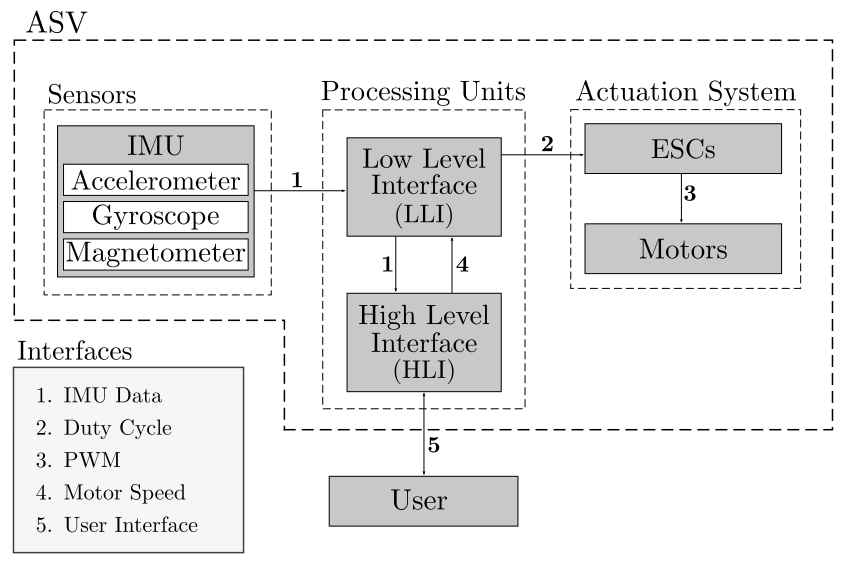
\includegraphics[width=.65\textwidth]{figures/systemDiagram4}
    \caption{A functional diagram of the given system.}
    \label{fig:systemDiagram}
\end{figure}
%
The main parts of the system are the actuators, the sensors and the control units, see \autoref{fig:systemDiagram}. The control unit gathers information from the IMU. This is handled by the Low Level Interface (LLI) which then sends it to the High Level Interface (HLI) where the control algorithms are implemented. The calculated actuation is then sent back to the LLI that sends the command to the actuation system. The ESCs (electronic speed controllers) then calculate the required signal to make the motors turn at the requested speed. 

This chapter briefly describes the main components of the surface vessel used in this project. Some additions to the existing systems are also presented.

